\newpage
\section{Calcolo combinatorio}

\subsection{Cardinalità insiemi}
Il calcolo combinatorio serve per dare delle risposte a domande come: quanti sono? In quanti modi? Quante possibili combinazioni?
Per questa forma di calcolo si fa molto utilizzo del concetto di cardinalità di un insieme.

\begin{definition}[Cardinalità]
La \textbf{cardinalità} di un insieme (finito) A è il numero dei suoi elementi e si indica con $\lvert A\rvert$.
\end{definition}

\begin{example}
$\lvert \{a,e,i,o,u\}\rvert = \lvert\{i,i,i,o,u,e,a,a\}\rvert = 5$ (Le ripetizioni non si contano)\\
$\lvert \O \rvert = 0$ \hspace{.7cm} $\lvert n\rvert = \lvert\{0,1,2,\ldots,n-1\}\rvert = n$ \hspace{.7cm} $\lvert 2\rvert = \lvert\{0,1\}\rvert = 2$
\end{example}

\begin{lemma}[Lemma-x]\label{lemma-x}
Dato un insieme $A$, sia $P = \{A_i\}_{i \in I}$ una partizione di $A$ quindi:
\begin{itemize}
    \item $\bigcup\limits_{i \in I}A_i = A$ (Punto (2) della definizione di partizione)
    \item $\forall i,j \in I . i\neq j \Longrightarrow A_i \cap A_j = \O$ (Punto (3) della definizione di partizione)
\end{itemize}
Allora vale che $\lvert A\rvert = \sum\limits_{i\in I}\lvert A_i\rvert$.
\end{lemma}
\begin{note}
Notare che nella proposizione sopra non è necessario che valga la condizione (1) di una partizione quindi che ($\forall i \in I . A_i \neq \O$), e ciò perché se consideriamo una partizione vuota essa non andrà ad influire sulla somma delle cardinalità avendo valore 0. 
\end{note}
\begin{demostration}
Per dimostrare questa proposizione supponiamo che $|A| \neq \sum\limits_{i\in I}|A_i|$, quindi $|A|$ sarà o maggiore o minore della sommatoria delle sue partizioni:
\begin{itemize}
    \item $|A| > \sum\limits_{i\in I}|A_i|$: questo caso contraddice il secondo punto della definizione di partizioni infatti fosse vero questo caso dovrebbe esistere un $a \in A$ che però $a \notin \forall i \: A_i$
    \item $|A| < \sum\limits_{i\in I}|A_i|$: questa casistica invece contraddice il terzo punto delle partizioni, infatti per far si che la cardinalità di A sia inferiore alla somma delle cardinalità delle partizioni dovrebbe esistere un $a \in A$ che contiamo due volte (ed è quindi presente in due partizioni distinte) ma questo farebbe si che $\exists A_i \neq A_j$ dove $A_i \cap A_j \neq \O$. $\blacksquare$
\end{itemize}
\end{demostration}

\subsubsection{Cardinalità di operazioni su insiemi}
\begin{proposition}
Per tutti gli insiemi A e B valgono i seguenti fatti:
\begin{enumerate}
    \item $|A| = |A\setminus B| + |A\cap B|$
    \item $|A \cup B| = |A\setminus B| + |A \cap B| + |B \setminus A|$
\end{enumerate}
\end{proposition}

\begin{demostration}
Dimostrazione con i diagrammi di eulero-vann della proprietà (1).
\end{demostration}
\begin{figure}[h!]
    \vspace{-5pt}
    \centering
    \begin{subfigure}{.3\textwidth}
        \centering
        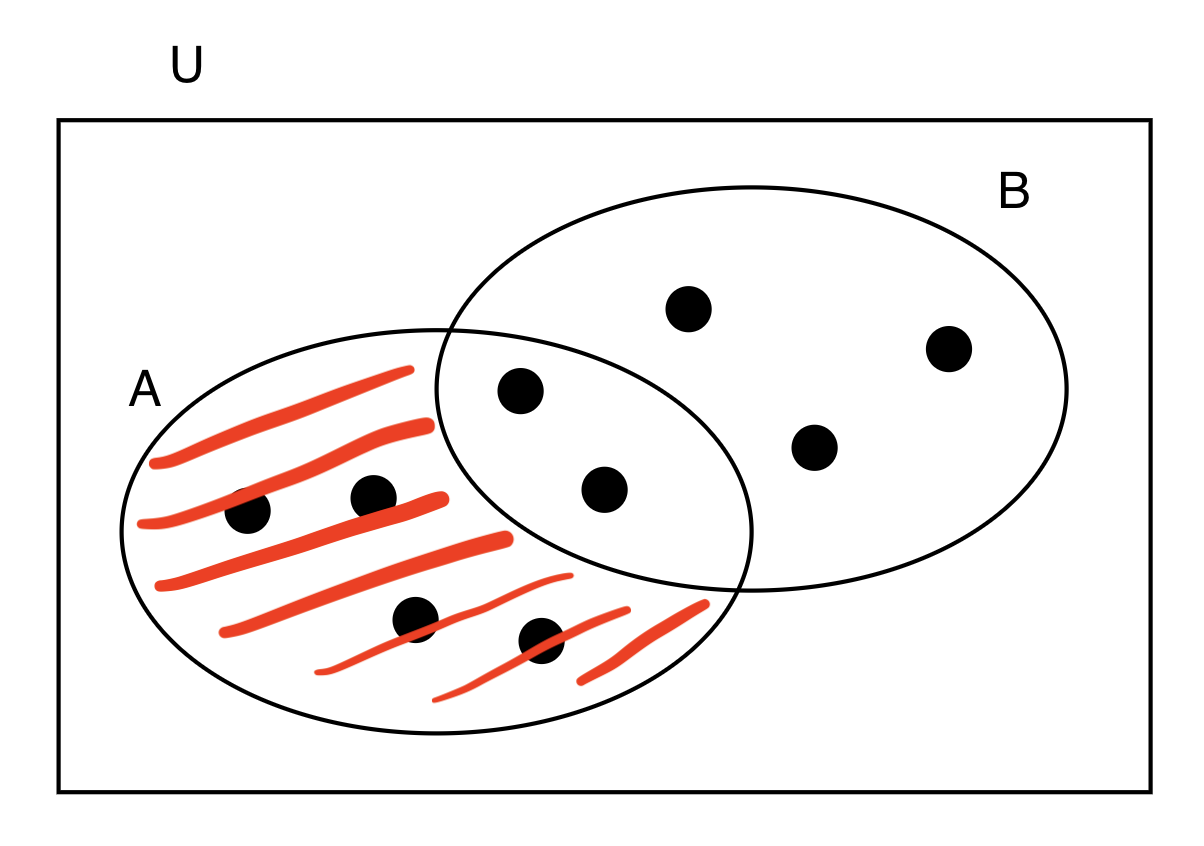
\includegraphics[width=4.2cm]{images/dim-prop-cardinalita-1.png}
        \caption{}
    \end{subfigure}
    \hfill
    \begin{subfigure}{.3\textwidth}
        \centering
        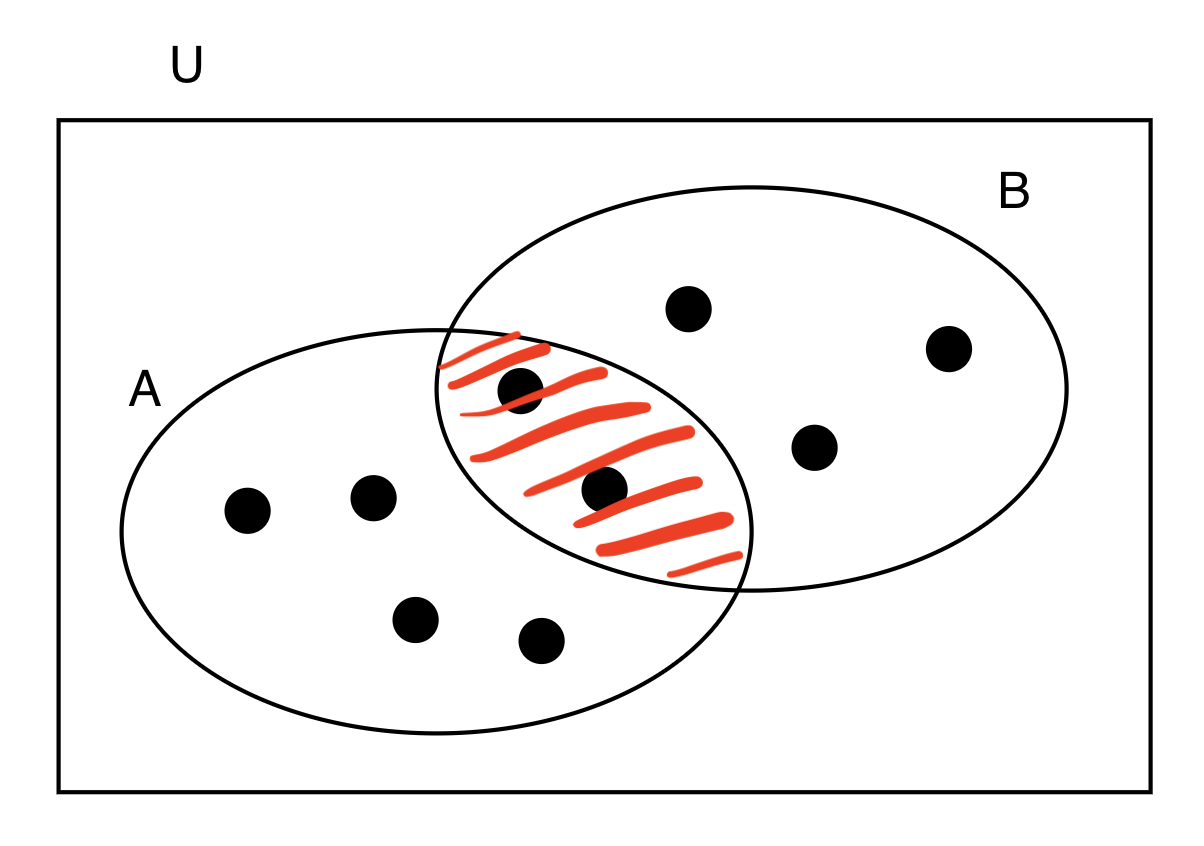
\includegraphics[width=4.2cm]{images/dim-prop-cardinalita-2.png}
        \caption{}
    \end{subfigure}
    \hfill
    \begin{subfigure}{.3\textwidth}
        \centering
        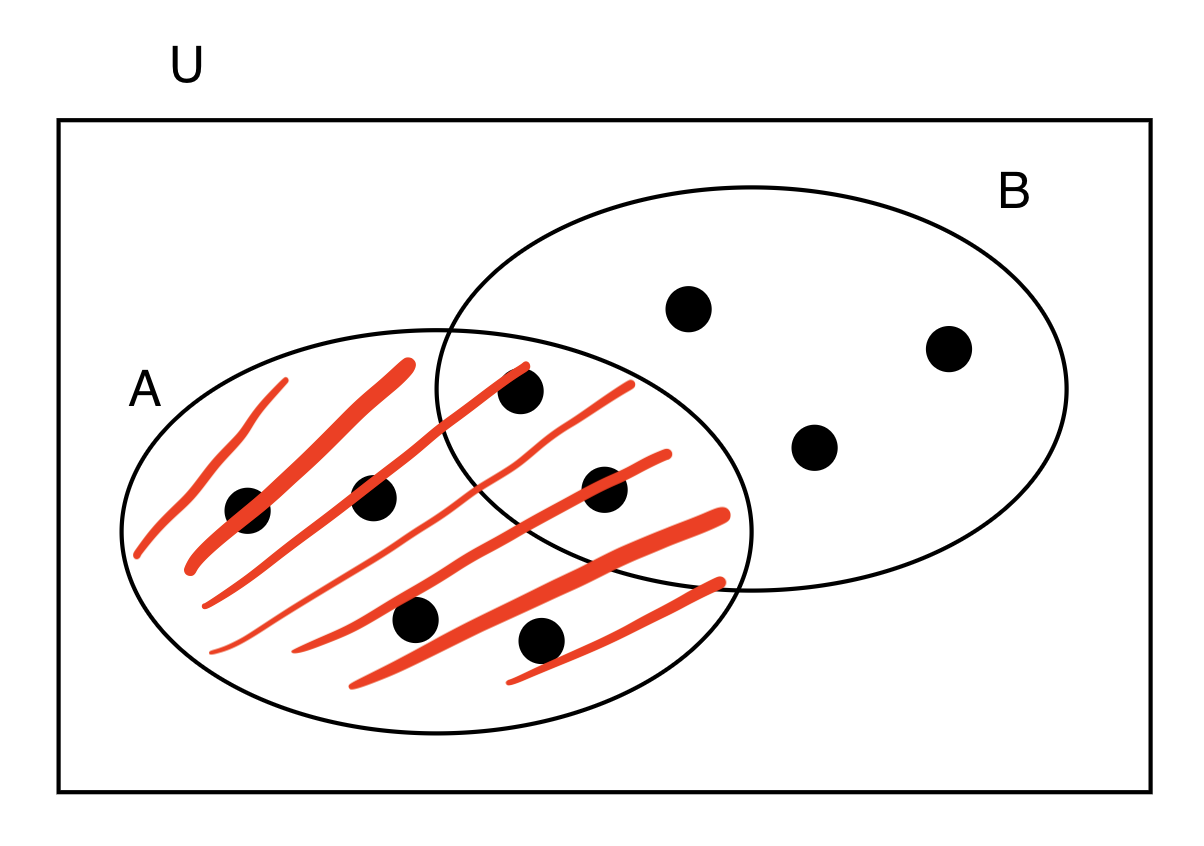
\includegraphics[width=4.2cm]{images/dim-prop-cardinalita-3.png}
        \caption{}
    \end{subfigure}
    \caption{In (a) $|A\setminus B|$, in (b) $|A\cap B|$, in (c) la somma di (a) e (b) uguale a $|A|$}
\end{figure}

\begin{corollar}
Per tutti gli insiemi A e b valgono i seguenti fatti:
\begin{enumerate}
    \item $|A \setminus B| = |A| - |A\cap B|$
    \item $|A \cup B| = |A| + |B| - |A \cap B|$
    \item $|A \cup B| \leq |A| + |B|$ e sono uguali $\Longleftrightarrow$ A e B sono disgiunti (lemma \ref{lemma-x})
    \item Se $B \subseteq A$ allora $|B| \leq |A|$
\end{enumerate}
\end{corollar}

\subsubsection{Principio di inclusione-esclusione}
La cardinalità dell'unione fra due insiemi si può definire come:
\begin{center}
    $|A \cup B| = |A| + |B| - |A \cap B|$
\end{center}
Questa formula può essere generalizzata a a 3 insiemi, essa si scrive come:
\begin{center}
    $|A \cup B \cup C| = |A| + |B| + |C| - |A\cap B| - |A\cap C| - |B \cap C| + |A \cap B \cap C|$
\end{center}
\begin{demostration}
Scriviamo $|A \cup B \cup C|$ come $|(A \cup B) \cup C|$ e prendiamo $(A \cup B)$ come fosse un unico insieme ed applichiamo la formula base.
\begin{itemize}
    \item $|(A \cup B) \cup C| = |(A \cup B)| + |C| - |(A \cup B) \cap C|$ (Ri-applichiamo la formula base su $(A \cup B)$).
    \item $= |A| + |B| - |A \cap B| + |C| - |(A \cup B) \cap C|$ (Scriviamo $|(A \cup B) \cap C|$ usando le proprietà degli insiemi).
    \item $= |A| + |B| - |A \cap B| + |C| - |(A \cap C) \cup (B \cap C)|$ (Usiamo lo stesso ragionamento iniziale su $|(A \cap C) \cup (B \cap C)|$).
    \item $= |A| + |B| - |A \cap B| + |C| - |(A \cap C) + (B \cap C)| - |(A \cap C) \cap (B \cap C)|$ (Riscriviamo $(A \cap C) \cap (B \cap C)$).
    \item $= |A| + |B| - |A \cap B| + |C| - |(A \cap C) + (B \cap C)| - |A \cap B \cap C|$ $\blacksquare$
\end{itemize}
\end{demostration}

\hspace{-15pt}Possiamo generalizzare ulteriormente questa formulala estendendola su $n$ insiemi .
\begin{definition}[Principio di inclusione-esclusione]
    Presi r insiemi $S_1, S_2,..., S_r$, abbiamo la seguente uguaglianza, dove $(-1)^i$ vale 1 se i è un numero pari e vale $-1$ se i è dispari:
    \begin{equation}
        \Biggl\lvert \bigcup\limits_{j=1}^r S_j \Biggr\rvert = \sum\limits_{I \subseteq \{1,2,...,r\}, I\neq \O }(-1)^{|I|+1} \Biggl\lvert\bigcap\limits_{i\in I}S_i\Biggr\rvert
    \end{equation}
\end{definition}
\hspace{-15pt}Questa formula spiegata a parole più semplici dice che:
\begin{itemize}
    \item Per ogni possibile sottoinsieme non vuoti $I \subseteq \{1,2,...,r\}$ consideriamo tutti gli insiemi $S_i$ tali che $i \in I$, e calcoliamo la cardinalità $n_i$ della loro intersezione.
    \item Sommiamo tutti i valori $n_I$ così calcolati per cui la cardinalità di $I$ è un numero dispari, e sottraiamo tutti i valori $n_I$ per cui la cardinalità di $I$ è un numero pari.
\end{itemize}
\begin{example}
Facciamo un esempio vedendo come si va a ricreare la stessa formula vista in precedenza con il caso $|A \cup B \cup C|$.
Prendiamo come $I \subseteq \{1,2,3\}$ prima $I = \{1\}$ poi $I = \{2\}$ e poi $I = \{3\}$ essi fanno si che $(-1)^{|I|+1} = 1$ quindi abbiamo che $|A| + |B| + |C|$ (Perché $\Biggl\lvert\bigcap\limits_{i\in I}S_i\Biggr\rvert$ con $I = \{1\}$, $I = \{2\}$, $I = \{3\}$ fa $|A|$ per il primo caso, $|B|$ per il secondo e $|C|$ per il terzo). \\\\
Continuiamo prendendo ora $I = \{1,2\}$ poi $I = \{2,3\}$ e poi $I = \{1,3\}$, in questo caso $(-1)^{|I|+1} = (-1)^{2+1} = -1$ quindi aggiungiamo le intersezioni ed otteniamo $|A| + |B| + |C| - |A \cap B| - |A \cap C| - |B \cap C|$. \\\\
Prendiamo ora l'ultimo sottoinsieme che ci manca e cioè $I = \{1,2,3\}$, questo fa si che $(-1)^{|I|+1} = (-1)^{3+1} = 1$ e così otteniamo $|A| + |B| + |C| - |A \cap B| - |A \cap C| - |B \cap C| + |A \cap B \cap C|$ che è la formula a vista in precedenza
\end{example}

\hspace{-15pt}Dal principio di inclusione-esclusione seguano come corollari il lemma \ref{lemma-x} visto sopra, la formula  $|A \cup B| = |A| + |B| - |A \cap B|$, e come visto nell'esempio anche la formula $|A \cup B \cup C| = |A| + |B| + |C| - |A\cap B| - |A\cap C| - |B \cap C| + |A \cap B \cap C|$.

\subsubsection{Cardinalità del prodotto cartesiano}
\begin{proposition}
Per tutti gli insiemi A,B vale che $|A \times B| = |A| \cdot |B|$.
\end{proposition}

\begin{demostration}
Per dimostrare questa proposizione usiamo il lemma \ref{lemma-x}. Innanzitutto definiamo $\forall a \in A$ una partizioni $S_a = \{(a,b) | b \in A\}$ in modo che $S_a \subseteq A \times B$. Vediamo anche che $|S_a| = |B|$. Ora se verifichiamo i due punti della lemma-x per vedere se possiamo applicare il lemma.
\begin{enumerate}
    \item $\bigcup\limits_{a \in A}S_a = A \times B$ è vera visto che $S_a$ si forma di coppie $(a_1, b_1), (a_1,b_2) ...$ per tutti gli elementi di $B$ quindi andando ad unire tutti gli $S_a$ (cioè le varianti con tutte le $a \in A$) abbiamo $A \times B$.
    \item $\forall a \neq a' S_a \cap S_a' = \O$ perché se cambiamo le $a$ avremo due insiemi completamente diversi.
\end{enumerate}
Vediamo dunque che l'insieme $S = \{S_a\}_{a \in A}$ (l'insieme di sotto insiemi)  è una partizione di $A \times B$. Quindi per il lemma-x abbiamo che:
\begin{center}
    $|A \times B| = \sum\limits_{a\in A}|S_a| = \sum\limits_{a \in A}|B| = |A| \cdot |B|$. $\blacksquare$
\end{center}
\end{demostration}

\begin{proposition}
Per ogni $n \geq 1$, per tutti gli insiemi $A_1, A_2, ...,A_{n-1}, A_{n}$ vale che:
\begin{center}
    $|A_1 \times A_2 \times ... \times A_{n-1} \times A_{n}| = |A_1| \cdot |A_2| \cdot ... \cdot |A_{n-1}| \cdot |A_{n}|$
\end{center}
\end{proposition}

\begin{demostration}
Dimostriamo questa proprietà per induzione.
\begin{enumerate}
    \item \underline{Caso base}: prendiamo $n = 1$, quindi $|A_1| = |A_1|$ verifica quindi la proprietà. Mentre se prendiamo $n = 2$, abbiamo che $|A_1 \times A_2| = |A_1| \cdot |A_2|$ che anche è dimostrata perché $|A_1| \cdot |A_n| = |A_1| \cdot |A_2|$.
    \item \underline{Passo induttivo}: Ora per induzione prendiamo come vera $P(n)$ e dimostriamo $P(n+1)$.\\
    Per dimostrare il passo induttivo ricordiamo che (a) $A \times B \times C \cong (A \times B) \times C$ e che (b) due insiemi hanno una biezione se e solo se hanno la stessa cardinalità.\\\\
    $P(n+1) = |A_1 \times A_2 \times ... \times A_{n} \times A_{n+1}|$ applicando la proprietà (a) e (b) riscritte sopra otteniamo $|(A_1 \times A_2 \times ... \times A_{n}) \times A_{n+1}|$ se poi scriviamo che $B = (A_1 \times A_2 \times ... \times A_{n})$ abbiamo che $|B \times A_{n+1}|$ che per caso base è uguale a $|B| \cdot |A_{n+1}| = |A_1| \cdot |A_2| \cdot ... \cdot |A_{n+1}|$. Abbiamo così concluso la dimostrazione $\blacksquare$.
\end{enumerate}
\end{demostration}

\begin{example}
Un esempio di cardinalità di prodotti cartesiani sono le targhe delle macchine italiane. \\
Le targhe hanno un formato XXCCCXX dove X è l'alfabeto (esclusi I,O,Q,U) e C sono le 10 cifre decimali. Quindi $|X| = 22$ e $|C| = 10$.
L'insieme delle possibili targhe di calcola dunque facendo $X \cdot X \cdot C \cdot C \cdot C \cdot X \cdot X = 22 \cdot 22 \cdot 10 \cdot 10 \cdot 10 \cdot 22 \cdot 22$.
\end{example}

\begin{corollar}
Sia $A^n$ l'insieme delle sequenze di lunghezza n su un inseme A. La sua cardinalità è $|A^n| = |A|^n$
\end{corollar}

\begin{example}
Esempio con la sequenza di caratteri ASCII esteso, di lunghezza n: con A = 256, quindi $|A^n| = 256^n$.
\end{example}
\begin{example}
Esempio con sequenza binaria di lunghezza n: con $A = \{0,1\} = 2$, abbiamo $|2^n| = 2^n$
\end{example}

\hspace{-15pt}Possiamo calcolare $|2^n|$ anche induttivamente. Sia $B(n)$ il numero di sequenze binarie di lunghezza $n$.
\begin{itemize}
    \item \underline{Caso base}: $B(0) = 1$, la sequenza vuota.
    \item \underline{Passo induttivo}: Ogni sequenza binaria di lunghezza $n+1$ + ottenuta aggiungendo 0 o 1 a una sequenza di lunghezza $n$, quindi: $B(n+1) = 2 \cdot B(n)$.
\end{itemize}

\newpage
\subsection{Relazioni e cardinalità}
\begin{proposition}\label{prop-rel-card-1}
Per tutti gli insiemi A, B e per tutte le relazioni $R: A \leftrightarrow B$ (quindi $R\subseteq A \times B$ e $0\geq |R|$ ed anche $|R| \leq |A| \cdot |B|$) vale che:
\begin{itemize}
    \item Se R è \textbf{totale} allora $|A|\leq |R|$.\\
    Perché se è totale tutti gli elementi dell'insieme di partenza hanno almeno un collegamento con l'insimeme di arrivo, perciò in R dovranno esserci almeno $|A|$ coppie ordinate o più (una per ciascun elemento di A che indica un collegamento).
    \item Se R è \textbf{univalente} allora $|R|\leq |A|$.\\
    Perché sia univalente tutti gli elementi di A devono collegarsi al più con uno di B dunque al massimo ci saranno $|A|$ coppie ordinate in R e non di più (sennò ci saranno per forsa ripetizioni di elementi di A).
    \item Se R è \textbf{surgettiva} allora $|B|\leq |R|$.
    Per surgettività discorso simili a quello del totale solo riferito agli elementi dell'insieme di arrivo.
    \item Se R è \textbf{iniettiva} allora $|R|\leq |B|$.
    Anche per iniettività discorso simili a quello di univalenza solo riferito all'insieme B.
\end{itemize}
\end{proposition}

\begin{note}\label{nota-1}
Nota anche che per far si che la relazione R sia una funzione $|R| = |A|$ e per far si che R sia biiezione allora $|R| = |A| \land |R| = |B|$ quindi $|A| = |B|$.
\end{note}

\subsubsection{Pigeonhole Principle}
Se abbiamo $n$ piccioni e li vogliamo collocare nelle $m$ caselle di una piccionaia, se $n > m$ allora almeno una casella conterrà due piccioni. Possiamo formalizzare questo enunciato nel seguente modo.
\begin{definition}[Pigeonhole Principle]
    Dati due insiemi P e C, se $|P| > |C|$ allora non esiste nessuna relazione $R: P \leftrightarrow C$ che sia totale e iniettiva. Infatti se esistesse una tale R, per la proposizione \ref{prop-rel-card-1} avremo $|P| \leq |R|$ (R totale) e $|R| \leq |C|$ (R iniettiva), da cui $|P| \leq |C|$ per transitività, contraddicendo l'ipotesi $|P| > |C|$.
\end{definition}

\subsubsection{Regola di biiezione}
Possiamo formalizzare quello scritto nella nota \ref{nota-1} riguardante la biiezione nel seguente corollario.
\begin{corollar}[Regola di biiezione]\label{regola-biiezione}
Per tutti gli insiemi A,B vale che se esiste una biiezione $R: A \leftrightarrow B$ allora $|A| = |B|$.
\end{corollar}

\begin{proposition}
Per ogni coppia di insiemi A e B vale che $|Fun(A,B)| = |B^{|A|}| = |B|^{|A|}$
\end{proposition}

\begin{demostration}
    Per dimostrare che $|Fun(A,B)| = |B|^{|A|}$ dimostriamo che esiste una biiezione fra $|Fun(A,B)|$ e $|B|^{|A|}$.\\
    Fun è totale e univalente, questo vuol dire che $\forall a \in A$ $f$ assegna esattamente 1 elemento di B.\\
    Possiamo scrivere $f: A \to B$ come $f: a_1, a_2, a_3, ..., a_{|A|}$ e $|B|^{|A|}$ come $b_1, b_2, b_3, ..., b_{|A|}$.\\
    Vediamo così che i due insiemi contengono lo stesso numero di elementi quindi può esistere una biiezione fra i due insiemi. $\blacksquare$
\end{demostration}

\begin{proposition}\label{proprosizione-reg-bii-1}
Per tutti gli insiemi A e per tutti i numeri naturali $n\in \mathbb{N}$ vale che; se $|A| = n$ allora $A \cong n$.
\end{proposition}
\hspace{-15pt}Questa proposizione è vera perché se consideriamo $n$ come un insieme di $n$ elementi (esempio $2 = \{0,1\}$) avendo A la stessa cardinalità di $n$ (ricorda che $|n| = n$) esisterà una biiezione fra i due insiemi.

\begin{theorem}
Per tutte le coppie di insiemi A e B vale che:
\begin{center}
    $A \cong B$ se e solo se $|A| = |B|$
\end{center}
\end{theorem}
\begin{demostration}
    Per dimostrare il teorema, trattandosi si un se e solo se, dobbiamo dimostrare i due versi della freccia:
    \begin{itemize}
        \item $A \cong B \Longrightarrow |A| = |B|$ immediato dal corollario \ref{regola-biiezione}.
        \item $A \cong B \Longleftarrow |A| = |B|$ assumiamo che $|A| = |B| = n$. Per la proposizione \ref{proprosizione-reg-bii-1} $A \cong n$ e $B \cong n$ quindi per le proprietà della biiezione $A \cong B$. $\blacksquare$
    \end{itemize}
\end{demostration}

\subsection{Permutazioni}
Fra i classici problemi del calcolo combinatorio abbiamo il caso in cui dato un insieme di $n$ oggetti, determinare quanti "raggruppamenti" diversi si possono avere disponendoli su $k$ posti. Da qui si possono usare formule diverse a seconda che l'ordine abbia importanza oppure no, ci possano essere ripetizioni oppure no.
\begin{definition}[Permutazione]
    Sia A un insieme con $|A| = n$. Una \textbf{permutazione} di A è una sequenza ordinata di tutti gli elementi di A: $a_0, a_1, ..., a_{n-1}$.
\end{definition}

\hspace{-15pt}Possiamo definire in maniera alternativa una permutazione di A come una funzione (una biiezione):
\begin{center}
    $\pi: A \to n$ con $n = |A|$
\end{center}
Infatti $\pi$ mappa ogni elemento di A con la posizione in cui si trova nella permutazione, è biiezione perché le permutazioni non ammettono ripetizioni e perché le permutazioni prevedono tutti gli elementi.

\begin{example}
Facciamo un esempio delle possibili permutazioni di $A = \{a,b,c,d\}$, $Perm(A)$ sono:\\
abcd - abdc - acbd - acdb - adbc - adcb - bacd - badc - bcad - bcda - bdac - bdca - ecc...\\
Il loro numero si calcola con $4! = 24$.\\
Se prendiamo un insieme $B = \{1,2,3,4\}$ o $S = \{$cuori, quadri, fiori, picche $\}$ il numero di permutazione è sempre $4! = 24$.
\end{example}

\begin{note}
Possiamo notare dall'esempio precedente che il numero di permutazioni dipende sola dal numero di elementi. Formalmente:
\begin{center}\vspace{-5pt}
    $|A| = |B| \Longrightarrow |Perm(A)| = |Perm(B)|$
\end{center}
E questo perché $Perm(A) \cong Bii(A,|A|) \cong Bii(B,|B|) \cong Perm(B)$
\end{note}

\begin{proposition}
Sia A un insieme di cardinalità $n > 0$. Allora ci sono esattamente
\begin{center}
    $P(n) = n!$
\end{center}
\end{proposition}
\hspace{-15pt}La dimostrazione per induzione è uguale a quella del fattoriale.

\subsubsection{Cardinalità delle biiezioni tra due insiemi}
Come visto in precedenza le permutazioni possono essere viste come una biiezione, da questa considerazione possiamo dimostrare che:
\begin{center}
    $Bii(A,B) = \begin{cases}
        0 & se \:\: |A| \neq |B|\\
        |A|! & se \:\: |A| = |B|\\
    \end{cases}$
\end{center}
Possiamo infatti immaginare che partendo dal primo elemento di A, $a_1$ esso avrà $|A|$ possibili scelte nell'insieme di partenza con cui essere in biiezione, l'elemento $a_2$ invece ne avrà $|A|$ meno l'elemento scelto per $a_1$ quindi $|A|-1$ e così per tutti gli elementi:\\
$a_1 \to |A|$, $a_2 \to |A| - 1$, $a_3 \to |A| - 2$, ..., $a_{|A|} \to 1$ \hspace{.5cm} Quindi $|Bii(A,B)| = |A| \cdot |A|-1 \cdot ... \cdot 1 = |A|!$

\subsubsection{Anagrammi e permutazioni con ripetizioni}
\begin{example}
Esempio di un anagramma: CERTOSA è anagramma di COSTARE. \\
CERTOSA ha $7! = 5040$ possibili anagrammi.\\\\
Se prendiamo invece $ANNA$ ha 6 anagrammi:\\
AANN \hspace{.5cm} ANAN \hspace{.5cm} ANNA \hspace{.5cm} NAAN \hspace{.5cm} NANA \hspace{.5cm} NNAA\\
Possiamo vedere dunque ch non possiamo usare la normale formula delle permutazioni, infatti $6 \neq 4! = 24$, avendo ANNA 2 caratteri ripetuti.\footnote{Ricorda che una parola non è un insieme ma è una sequenza di lettere, e può quindi contenere ripetizioni}
\end{example}

\begin{proposition}[Permutazioni con ripetizioni]
Sia $S = s_1, s_2, ..., s_k$ una sequenza di elementi di un insieme $A = \{a_1, a_2, ..., a_n\}$ di cardinalità n, ogni elemento di A può comparire 0 o più volte. Inoltre per ogni $i \in \{1,2,..., n\}$ sia $c_i$ il numero di volte che l'elemento $a_i$ compare nelle sequenza S. Il numero di \textbf{permutazioni con ripetizioni} della sequenza è dato da:
\begin{equation}
    \frac{\displaystyle k!}{\displaystyle c_1! \cdot c_2! \cdot ... \cdot c_n!}
\end{equation}
\end{proposition}

\subsection{Disposizioni}
\begin{definition}[Disposizioni]
    Dato un insieme finito A con $|A| = n$ e un intero $k \leq n$, una \textbf{disposizione} degli elementi d A in k posti è una sequenza ordinata $a_1, ..., a_k$.
\end{definition}

\begin{example}
Se per esempio prendiamo $A = \{a,b,c,d,e\}$ e $k = 2$ (quindi 2 posti dove disporre gli elementi dell'insieme) abbiamo 20 possibili disposizioni:\\
ab, ae, bd, cb, da, de, ec, ac, ba, be, cd, db, ea, ed, ad, bc, ca, ce, dc, eb
\end{example}

\begin{proposition}
Sia A un insieme di cardinalità $n > 0$ e k tale che $0 < k \leq n$. Allora ci sono esattamente:
\begin{equation}
    D(n,k) = \frac{\displaystyle n!}{\displaystyle (n - k)!}
\end{equation}
disposizioni degli elementi di A in k posti.
\end{proposition}
\hspace{-15pt}Questa formula è semplicemente ricavata da una permutazione al numeratore (che però da sola conterrebbe potenzialmente anche elementi in posizioni extra) e da le posizione da non conteggiare al denominatore.

\begin{demostration}
    Dimostriamo per induzione su k questa proprietà.
    \begin{enumerate}
        \item \underline{Caso base:} Per $k=1$ abbiamo $D(n,1) = n = \frac{\displaystyle n \cdot (n - 1)!}{\displaystyle (n - 1)!}$.
        \item \underline{Passo induttivo:} Assumiamo vero $P(k)$ e dimostriamo $P(k+1)$. Quindi $D(n,k) = \frac{\displaystyle n!}{\displaystyle (n - k)!}$ la consideriamo vera mentre noi dobbiamo dimostrare: $D(n,k+1) = \frac{\displaystyle n!}{\displaystyle (n - (k + 1))!}$\\\\
        $D(n,k+1) = \frac{\displaystyle n!}{\displaystyle (n - k)!} \cdot (n-k) = \frac{\displaystyle n!}{\displaystyle (n - (k + 1))!}$. \\\\
        (Perché andando ad aggiungere un posto "k+1" dovremo mantenere una posizione in più nella permutazione nel quale si sceglierà fra n-k elementi).$\blacksquare$
    \end{enumerate}
\end{demostration}

\subsection{Combinazioni}
\begin{definition}[Combinazioni]
    Sia A un insieme di cardinalità n e sia $k \leq n$ un numero naturale. Una \textbf{combinazione} di k elementi di A è un k-insieme di A, cioè un sottoinsieme di A di cardinalità k. L'insieme di tutte le combinazioni di k elementi di A è quindi denotato con $\mathcal{P}_k(A).$
\end{definition}

\begin{example}
Prendiamo per esempio l'insieme $A = \{a,b,c,d,e\}$, le 10 combinazioni possibili sono:
abc, abe, ace, bcd, bde, abd, acd, ade, bce, cde.
\end{example}

\begin{note}
Nota che nelle combinazioni non ci interessa l'ordine degli elementi $\{a,b,c\} = \{c,b,e\}$.
\end{note}

\begin{definition}[Coefficiente binomiale]
Dato un insieme A di cardinalità n, il numero di combinazioni di k elementi è chiamo \textbf{coefficiente binomiale}.
\begin{equation}
    \binom{n}{k} = \frac{\displaystyle n!}{\displaystyle k! \cdot (n - k)!}
\end{equation}
\end{definition}

\hspace{-15pt}Per giustificare questa formula partiamo dal fatto che per disporre n elementi in k posti si deve applicare una disposizione del tipo $D(n,k) = \frac{n!}{(n - k)!}$, essendo una disposizioni però teniamo conto della posizione degli elementi, andando così a creare più possibilità rispetto alle combinazioni dove non teniamo conto delle posizioni. Per eliminare dunque le possibilità extra andiamo a dividere per le permutazioni degli n elementi $P(n) = n!$ otteniamo dunque:
\begin{center}
    $\binom{n}{k} = \frac{D(n,k)}{P(k)} = \frac{\frac{n!}{(n-k)!}}{k!} = \frac{n!}{k! \cdot (n - k)!}$
\end{center}

\begin{demostration}
    Dimostrazione per induzione del coefficiente binomiale:
    \begin{enumerate}
        \item \underline{Caso base:} Definiamo due casi base.
        \[\binom{n}{0} = \frac{n!}{0! \cdot n!} = 1 \hspace{.3cm}\text{e}\hspace{.3cm} \binom{n}{n} = \frac{n!}{n! \cdot 0!} = 1\]
        \item \underline{Passo induttivo:} Prendiamo come vera l'ipotesi induttiva $P(k)$ e dimostriamo $P(k + 1)$. Dobbiamo dunque dimostrare la validità della formula: \[\frac{n!}{(k+1)! \cdot (n - (k+1))!}\]
        $\binom{n}{k} = \binom{n - 1}{k} + \binom{n - 1}{k - 1} = \frac{(n-1)!}{k! (n - 1 - k)} + \frac{(n-1)!}{(k - 1)! (n - k)}$ (Spiegazioni della formula usata su dispense).\\\\
        $= \frac{(n-1)!}{(k-1)!(n-1-k))} \cdot \bigl(\frac{1}{k} + \frac{1}{n-k} \bigr)$ (Raccogliamo le due frazioni).\\\\
        $= \frac{(n-1)!}{(k-1)!(n-1-k))} \cdot \frac{n}{k(n-k)} = \frac{n!}{k!(n-k)!}$ (Risolviamo l'equazione). $\blacksquare$
    \end{enumerate}
\end{demostration}

\begin{example}
Calcoliamo le combinazioni di 3 elementi di $A = \{a,b,c,d,e\}$.\\
$\binom{5}{3} = \frac{5!}{ 3! \cdot (5 - 3)!} = \frac{5!}{5! \cdot 2!} = \frac{20}{2} = 10$
\end{example}

\subsection{Contare sui grafi}
\subsubsection{Grafi non orientati}
Partiamo ponendoci una domanda. Dati i nodi $\{1,2,...,n\}$, quanti grafi diversi possiamo comporre?\\
Chiamiamo $G_n$ l'insieme di grafi con $n$ nodi, quindi quello che cerchiamo è la sua cardinalità. Per riuscire a contare tutte le possibilità dobbiamo considerare quanti grafi possono esistere dando un numero di archi.
\begin{example}
Prendiamo $n=3$ nodi e calcoliamo:\\
Quanti grafi esistono con 0 archi? Esiste 1 grafo.\\
Se invece vogliamo quanti grafi esistono con 1 arco questi sono 3.\\
Possiamo continuare vino ad il caso con 3 archi perché andando a tutti le casistiche con archi $>3$ abbiamo che non esistono grafi.
\end{example}
\hspace{-15pt}Possiamo notare che nel caso di $n=3$ nodi e 0 archi il calcolo si bassa su fare $\binom{n}{0}$ mentre per $n=3$ e 3 archi abbiamo $\binom{n}{1}$, cosi anche per tutti i casi con numero di archi minori o uguali a $n$. Vediamo dunque che il modo di calcolare il numero di grafi con $n$ nodi è:
\[|G_n| = \sum_{i \in \{0,...,m_{max}\}}\binom{m_{max}}{i} \text{ con } m_{max} = \frac{n(n-1)}{2} \text{ il numero massimo di archi}\] 
Esiste però un metodo alternativo per contare i grafi dati $n$ nodi, e si passa su valutare, per ogni arco se includerlo oppure no, infatti da questo ragionamento vediamo che per ogni arco abbiamo due scelte, da qui possiamo vedere che per calcolare tutte i grafi possibili basta fare $2^m \text{ con } m = \frac{n(n-1)}{2}$.\\\\
Il conteggio di tutti i possibili sottoinsiemi di $m$ elementi è anche noto come insieme delle parti, questo ci aiuta anche a dimostrare che:
\[\mathcal{P}(m_{max}) = \sum_{i \in \{0,...,m_{max}\}}\binom{m_{max}}{i} = 2^{m_{max}}\]
Come conseguenza possiamo notare che c'è una biezione fra $\mathcal{P}(m_{max}) \cong fun(m_{max},2) \cong \{0,1\}^{m_{max}}$.\\
E vediamo anche due proprietà del coefficente bionomiale che vengono di conseguenza:
\[\sum_{i \in \{0,...,k\}}\binom{k}{i} = 2^{k}, \text{ e quindi } \forall \: k>0,i\geq 0 \binom{k}{i} < 2^k\]

\subsubsection{Grafi orientati}
Per i grafi orientati possiamo usare la stessa logica, l'unica cosa è che dobbiamo contare ogni arco due volte, avendo per ogni 2 nodi due possibili archi che li collegano, e dobbiamo anche considerare i cappi; questo vuol dire che abbiamo $n^2$ possibili archi.
\begin{theorem}
Esistono $2^{\frac{n(n-1)}{2}}$ grafi non orientati su $n$ nodi, e $2^{n^2}$ grafi orientati su $n$ nodi.
\end{theorem}